\documentclass[12pt,a4paper]{article}
\usepackage{amsmath,amscd,amsbsy,amssymb,latexsym,url,bm,amsthm}
\usepackage{epsfig,graphicx,subfigure}
\usepackage{enumitem,balance}
\usepackage{wrapfig}
\usepackage{mathrsfs,euscript}
\usepackage[usenames]{xcolor}
\usepackage{hyperref}
\usepackage[vlined,ruled,linesnumbered]{algorithm2e}
\hypersetup{colorlinks=true,linkcolor=black}

\newtheorem{theorem}{Theorem}
\newtheorem{lemma}[theorem]{Lemma}
\newtheorem{proposition}[theorem]{Proposition}
\newtheorem{corollary}[theorem]{Corollary}
\newtheorem{exercise}{Exercise}
\newtheorem*{solution}{Solution}
\newtheorem{definition}{Definition}
\theoremstyle{definition}

\renewcommand{\thefootnote}{\fnsymbol{footnote}}

\newcommand{\postscript}[2]
 {\setlength{\epsfxsize}{#2\hsize}
  \centerline{\epsfbox{#1}}}

\renewcommand{\baselinestretch}{1.0}

\setlength{\oddsidemargin}{-0.365in}
\setlength{\evensidemargin}{-0.365in}
\setlength{\topmargin}{-0.3in}
\setlength{\headheight}{0in}
\setlength{\headsep}{0in}
\setlength{\textheight}{10.1in}
\setlength{\textwidth}{7in}
\makeatletter \renewenvironment{proof}[1][Proof] {\par\pushQED{\qed}\normalfont\topsep6\p@\@plus6\p@\relax\trivlist\item[\hskip\labelsep\bfseries#1\@addpunct{.}]\ignorespaces}{\popQED\endtrivlist\@endpefalse} \makeatother
\makeatletter
\renewenvironment{solution}[1][Solution] {\par\pushQED{\qed}\normalfont\topsep6\p@\@plus6\p@\relax\trivlist\item[\hskip\labelsep\bfseries#1\@addpunct{.}]\ignorespaces}{\popQED\endtrivlist\@endpefalse} \makeatother

\begin{document}
\noindent

%========================================================================
\noindent\framebox[\linewidth]{\shortstack[c]{
\Large{\textbf{Lab04-Programming and Amortized Analysis}}\vspace{1mm}\\
Algorithm and Complexity, Xiaofeng Gao, Spring 2022.}}
\begin{center}
\footnotesize{\color{red}$*$ If there is any problem, please contact TA Jialin Lyu.}

% Please write down your name, student id and email.
\footnotesize{\color{blue}$*$ Name: Zhenran Xiao  \quad Student ID: 520030910281 \quad Email: xiaozhenran@sjtu.edu.cn}
\end{center}



\begin{enumerate}
    \item
    Assume we have a set of arrays $A_0, A_1, A_2,\cdots$, where the $i^{th}$ array $A_i$ has a length of $3^i$. Whenever an element is inserted into the arrays, we always intend to insert it into $A_0$. If $A_0$ is full, we should first pop the element in $A_0$ off and insert it into $A_1$, and then insert the new element in $A_0$. (Thus, if $A_{i}$ is already full, we should recursively pop all its members off and insert them into  $A_{i+1}$ until we find an empty array to store the new element.) An illustrative example is shown in Figure \ref{Fig-1}. Inserting or popping an element takes $O(1)$ time.

	\begin{figure}[!htbp]
	\centering
	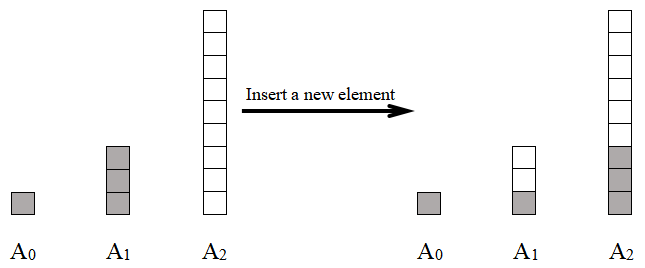
\includegraphics[width=0.5\textwidth]{Fig-1.png}
	\caption{An example of making room for one new element in the set of arrays.}
	\label{Fig-1}
	\end{figure}

    \begin{enumerate}
        \item
        In the worst case, how long does it take to add a new element into the set of arrays containing $n$ elements?
        \item
        Prove that the amortized cost of adding an element is $O(\log n)$ by \emph{Aggregation Analysis}.
        \item
        If each array $A_i$ is required to be sorted but elements in different arrays have no relationship with each other, what is the amortized cost of adding an element if the comparison between two elements also takes $O(1)$ time?
    \end{enumerate}

\begin{solution}
	\quad \\
	\begin{enumerate}
		\item 
		The worst case is the old $n$ elements fill up the first $i$ arrays. $n = \sum_{k = 0}^{i} 3^i = \frac{3^{i + 1} - 1}{2}$. \\
		If we want to add a new element into the set of arrays, for each $k$ from $0$ to $i$, we should pop all the elements in $A_{k}$ off and insert them into $A_{k+1}$. Finally insert the new element into $A_0$.
		\[
		\sharp pop + \sharp insert = n + (n + 1) = 2n + 1 \sim O(n)
		\]
		So it takes $O(n)$ time.
		\item
		Assume that the cost of $k$th adding is $C_k$, the $k$th element has been operated for $p_k$ times. 
		\[
		\begin{aligned}
			\sum_{k=1}^{n} C_k &= \sharp pop + \sharp insert \\
			&= \sum_{k=1}^{n} p_k 
		\end{aligned}
		\]
		When there are $n$ elements in the set of arrays. The fisrt added one is in the $A_i$, $i = \log_3 (2n + 1) - 1$ or $\log_3 (2n + 1)$. So
		\[
		p_1 = \sharp insert_1 + \sharp pop_1 = i + i - 1 \leq 2\log_3 (2n + 1)
		\]
		Therefore, 
		\[
		\begin{aligned}
			\sum_{k=1}^{n} C_k &= \sharp pop + \sharp insert \\
			&= \sum_{k=1}^{n} p_k \\
			&\leq n\cdot 2\log_3 (2n + 1)
		\end{aligned}
		\]
		The amortized cost of adding a new element is
		\[
		T(n) = \frac{\sum_{k=1}^{n} C_k}{n} \leq 2\log_3 (2n + 1) \sim O(\log n)
		\]
		\item 
		After adding, sorting each array takes $O(3^k\log 3^k)$ time. Sorting all the arrays takes
		$O(\sum_{k = 0}^{i} \log 3 \cdot k3^k) \sim O(n\log n)$ time. \\
		So the amortized cost is 
		\[
			T(n) \leq O(\log n) + O(n\log n) \sim O(n\log n)
		\]
		
		
		
	\end{enumerate}
\end{solution}

    \item
    \textit{Machine Assignment.} A company intends to import $100$ machines at the beginning of $2022$, with a proper combination of the following $2$ production modes:
    \begin{itemize}
    \item \textbf{High workload mode:} When the machine runs under high load, the annual profit of each machine is $100$ thousand yuan, and the machine damage rate is $0.25$ per year;
    \item \textbf{Low workload mode:} When the machine runs under low load, the annual profit of each machine is $80$ thousand yuan, and the machine damage rate is $0.1$ per year;
    \end{itemize}

    \begin{enumerate}
    \item
    Consider a $2$-year short-term production plan, please design a scheme of assignment from $2022$ to $2023$ which maximizes the overall profit at the end of $2023$, formulate a linear programming model and give its solving process and optimal solution with necessary explanations.

    \item
    Transform your LP model in (a) into its standard form and slack form.

    \item
    Transform your LP model in (a) into its dual form.

    \end{enumerate}

\begin{solution}
	\quad \\
	\begin{enumerate}
		\item 
		Suppose in 2022 $x_1$ machines work under high load, $x_2$ machines work under low load; in 2023 $x_3$ machines work under high load, $x_4$ machines work under low load. \\
		According to the settings, we have
		\begin{itemize}
			\item At the beginning of 2022, there are 100 machines: $x_1 + x_2 \leq 100$
			\item At the beginning of 2023,  there are $100 - 0.25x_1 - 0.1 x_2$ machines: $x_3 + x_4 \leq 100 - 0.25x_1 - 0.1 x_2$
			\item Nonnegative machine: $x_1, x_2, x_3, x_4 \geq 0$
		\end{itemize}
		Maximizeing the overall profit: 
		\[
		max\quad f(x_1, x_2, x_3, x_4) = 100x_1 + 80x_2 + 100x_3 + 80x_4
		\]
		Linear programming model:
		\[
		\begin{aligned}
			&max &f(x_1, x_2, x_3, x_4) &= 100x_1 + 80x_2 + 100x_3 + 80x_4 \\
			&s.t. &x_1 + x_2 &\leq 100 \\
			& &x_3 + x_4 &\leq 100 - 0.25x_1 - 0.1 x_2 \\
			& &x_1, x_2, x_3, x_4 &\geq 0 \\
		\end{aligned}
		\]
		If we want maximuize the profit, we should make all machines busy. So we can let 
		\[
		\begin{aligned}
			x_1 + x_2 &= 100 \\
			x_3 + x_4 &= 100 - 0.25x_1 - 0.1 x_2 \\
		\end{aligned}
		\]
		We put $x_2 = 100 - x_1$ and $x_4 = 100 - 0.25x_1 - 0.1(100 - x_1) - x_3$ into the origin LP model. Then we can obtain a new LP model:
		\[
		\begin{aligned}
			&max &f(x_1, x_3) &= 8x_1 + 20x_3 + 15200 \\
			&s.t. &x_1 &\leq 100 \\
			& &0.15x_1 + x_3 &\leq 90 \\
			& &x_1, x_3 &\geq 0 \\
		\end{aligned}
		\]   
		We can establish Coordinate system $x_3-x_1$. Constrains form the feasible region: 
		$$ 
		\left\{
		\begin{aligned}
			x_1 &\geq 0 \\
			x_1 &\leq 100 \\
			x_3 &\geq 0 \\
			x_3 &\leq 90 - 0.15x_1 \\
		\end{aligned}
		\right\}
		$$
		Let $p$ represent the profit. We can use the line $x_3 = -0.4x_1 + 0.05p - 760$ to find the optimum point. It is $(100, 75)$. \\
		Therefore the optimal scheme is that in 2022 $100$ machines work under high load, $0$ machine works under low load; in 2023 $75$ machines work under high load, $0$ machine works under low load. The overall profit is $100\times 100 + 100\times 75 = 17500$ thousand yuan. \\
		
		\item 
		Transform to standard form: 
		\[
		\begin{aligned}
			&max &f(x_1, x_2, x_3, x_4) &= 100x_1 + 80x_2 + 100x_3 + 80x_4 \\
			&s.t. &x_1 + x_2 &\leq 100 \\
			& &x_3 + x_4 + 0.25x_1 + 0.1x_2 &\leq 100 \\
			& &x_1, x_2, x_3, x_4 &\geq 0 \\
		\end{aligned}
		\]
		Transform to slack form: 
		\[
		\begin{aligned}
			&max &f(x_1, x_2, x_3, x_4) &= 100x_1 + 80x_2 + 100x_3 + 80x_4 \\
			&s.t. &x_1 + x_2 + x_5 &= 100 \\
			& &x_3 + x_4 + 0.25x_1 + 0.1x_2 + x_6 &= 100 \\
			& &x_1, x_2, x_3, x_4, x_5, x_6&\geq 0 \\
		\end{aligned}
		\]
		$x_5$, $x_6$ are slack variables. \\
		
		\item 
		Transfrom to dual from: \\
		Set the multiplier $y_1$ and $y_2$. $y_1, y_2 \geq 0$ to ensure no flipping from $\leq$ to $\geq$ in constraints. Multiply horizontally and add vertically, we obtain
		\[
		(y_1 + 0.25y_2)x_1 + (y_1 + 0.1y_2)x_2 + y_2x_3 + y_2x_4 \leq 100y_1 + 100y_2
		\]
		We want the left-hand side to look like out objective function $100x_1 + 80x_2 + 100x_3 + 80x_4$, so that the right-hand side becomes an upper bound on the objective function.
		\[
		100x_1 + 80x_2 + 100x_3 + 80x_4 \leq 100y_1 + 100y_2 \quad if \left\{
		\begin{aligned}
			y_1, y_2 &\geq 0 \\
			y_1 + 0.25y_2 &\geq 100 \\
			y_1 + 0.1y_2 &\geq 80 \\
			y_2 &\geq 100 \\
			y_2 &\geq 80 \\
		\end{aligned}
		\right\}
		\]
		The dual form:
		\[
		\begin{aligned}
			&min &g(y_1, y_2) &= 100y_1 \\
			&s.t. &y_1 + 0.25y_2 &\geq 100 \\
			& &y_1 + 0.1y_2 &\geq 80 \\
			& &y_2 &\geq 100 \\
			& &y_2 &\geq 80 \\
			& &y_1, y_2 &\geq 0 \\
		\end{aligned}
		\]
		
	\end{enumerate}
\end{solution}

    \item
    \textit{Collect Jingye Fu.} Collecting \emph{Five Fortune Cards} was considered as a new tradition of most of Chinese people during Spring Festival. Little Gyro is planning to collect \emph{Five Fortune Cards} on Alipay in $2022$.

    As the product manager Hua Guan explains, aside from scanning the specific Chinese Character \emph{Fu} to gain \emph{Jingye Fu}, which is one of \emph{Fortune Cards} usually hard to get, users also can using a \emph{Sticky Card} to copy your friend��s \emph{Jingye Fu}. For each friend, users only have \textbf{one} chance to use the \emph{Sticky Card}. After using a \emph{Sticky Card}, you will obtain the \emph{Fortune Card} which you stick with, and it's always the same type \emph{Fortune Card} as your friend's already have. But whether you get \emph{Jingye Fu} or not, this card will disappear. To enhance the possibility of getting \emph{Jingye Fu}, Hua Guan suggests that you should find your friend who has many \emph{Fortune Cards}, because the system will accumulate your \emph{Fortune Value}, which is calculated by adding the total number of your friends \emph{Fortune Cards} who you stick with. So Hua Guan considers that, the more \emph{Fortune Cards} your friends have, the more \emph{Fortune Value} you will accumulated, and the more possibility you will get \emph{Jingye Fu}.

    \begin{figure}[!htbp]
	\centering
	
\includegraphics[width=0.5\textwidth]{Fig-2.jpeg}
	\caption{The picture of \emph{Jingye Fu}.}
	\label{Fig-2}
	\end{figure}

    After known these regulations, Little Gyro thinks that he wants to get \textbf{one} \emph{Jingye Fu} \textbf{not under than} the possibility $P$, as well as get more \emph{Fortune Value} as possible. So Little Gyro makes a list and collects his friends�� information about the amount of \emph{Fortune Card} and \emph{Jingye Fu} they already have. But the amount of \emph{Sticky Card} was limited, Little Gyro wants to know which friend he should stick with. Can you help him?

    \textbf{It��s guaranteed that Little Gyro will definitely get a \emph{Fortune Card} when using a \emph{Sticky Card}.}

    \textbf{Input Specification:}

    There are multiple test cases. The first line of the input is an integer $T (1 \leq T \leq 10)$, indicating the number of test cases. Then $T$ test cases follow.

    The first line of each test case contains two integers $n,m (1 \leq n \leq 1000, 1 \leq m \leq 10)$ and one floating point number $P (0 \leq P \leq 1)$, indicating the number of friends, the number of \emph{Sticky Card} and the least possibility Little Gyro will get one \emph{Jingye Fu}, respectively.

    The following $n$ lines describe the information of Little Gyro��s friends, numbered from $1$ to $n$. The $(i+1)$-th line contains two positive integers $t_i$ and $h_i (1 \leq h_i \leq t_i \leq 100)$, representing the total number of \emph{Fortune Card} and the number of \emph{Jingye Fu} the $i$-th friend has, respectively.

    \textbf{Output Specification:}

    For each test case output two lines, the first line consists one integer, indicating the maximum \emph{Fortune Value}. The second line consists at most $m$ numbers, indicating the number of Little Gyro��s friends (within the ascending order) who stuck with.

    If there exists more than one proper solutions, output the solution with the maximum \emph{Fortune Value}. And if there is no solution, output "No Solution" (without quotes) in one line instead.

    \textbf{It��s guaranteed that the proper solutions with the maximum \emph{Fortune Value} is unique.}

    \fbox{
    \begin{minipage}[t]{0.2\textwidth}
    \textbf{Sample Input:}
	
	2 \\ 3 2 0.75 \\ 5 2 \\ 10 4 \\ 5 3 \\ 3 2 0.50 \\ 20 3 \\ 10 2 \\ 5 1
    \end{minipage}
    \begin{minipage}[t]{0.2\textwidth}
    \textbf{Sample Output: }
	
	15 \\ 2 3 \\ No Solution
    \end{minipage}}
    \hspace{1cm}
    \begin{minipage}[t]{0.45\textwidth}
    \textbf{Remark:} The input data \texttt{Lab04-JingyeFu.in} (sample test cases only) and the template code \texttt{Lab04-JingyeFu.cpp} are attached on the course webpage. Please include your \texttt{Lab04-JingyeFu.cpp} file in your uploaded .rar or .zip file.
    \end{minipage}

    \textbf{Hint:}

    In the first sample, Little Gyro can choose $1$ and $3$ or $2$ and $3$ to stick with in order to achieve the possibility $0.75$. So the maximum \emph{Fortune Value} is $15$.

    In the second sample, Little Gyro can not find any ways to achieve the possibility $0.50$.

	\begin{enumerate}
    \item
    Please briefly describe your algorithm and analyze its time complexity and space complexity. Is the greedy algorithm solvable? If it can be solved by greedy algorithm, please explain the reason. If not, please give a counterexample.

    \item
    Try to write a C/C++ code to solve this problem, you only need to complete the \texttt{TODO} part in \texttt{Lab04-JingyeFu.cpp}. Your program will be judged by the online judge system, including several test cases, half for the test data which equivalent to the sample test case, and another half for other corner and huge test cases.
    \end{enumerate}

 \begin{solution}
	\quad \\
	\begin{enumerate}
		\item 
		My alogrithm: For all the ways of picking m friends out of n friends, calculate the Fortune Value and the possiblility P. Use the bigger Fortune Value with eligible P to update the solution set. Finally we obtain the optimal solution. \\
		Use DFS to obtain all the ways of picking m friends out of n, namely using recursion to realize combinatorial enumeration. \\
		Time complexity:  $O(m \binom{n}{m})$. \\
		Space complexity: $O(n + m)$ \\
		
		About greedy algorithm: 
		\begin{itemize}
			\item 
			If the greedy algorithm is: Find the combination with the biggest Fortune Value, check whether its P is eligible. If not, find the combination with the second biggest Fortune Value. Until it find a combination with an eligible P. This combination is the optimal solution. \\   
			Then the greedy algorithm is solvable. But it is not easy to find the combination with the $k$ biggest Fortune Value. 
			
			\item 
			If the greedy algorithm is just choosing m friends with m biggest Fortune Values, then it is not solvable. The second sample in the sample input can be a counterexample. \\
		\end{itemize}
		
		\item 
		Please check it in \texttt{Lab04-JingyeFu.cpp}.
	\end{enumerate}
\end{solution}

\end{enumerate}

\vspace{20pt}

\textbf{Remark:} You need to include your .pdf and .tex files in your uploaded .rar or .zip file.

%========================================================================
\end{document}
